\section{How the Rule Policy Works}
\label{sec:controller}
At each control step, the policy follows a simple principle: \emph{look at the current scene, decide which part of the job is next, make a small movement, and check what actually happened}. This is a feedback controller rather than a fixed prerecorded motion. Layered feedback control and visual servoing are established ideas in robotics~\cite{brooks,servo}; our work applies them to the particular geometry and scoring rules of this cookie task.

\begin{figure*}[t]
\centering
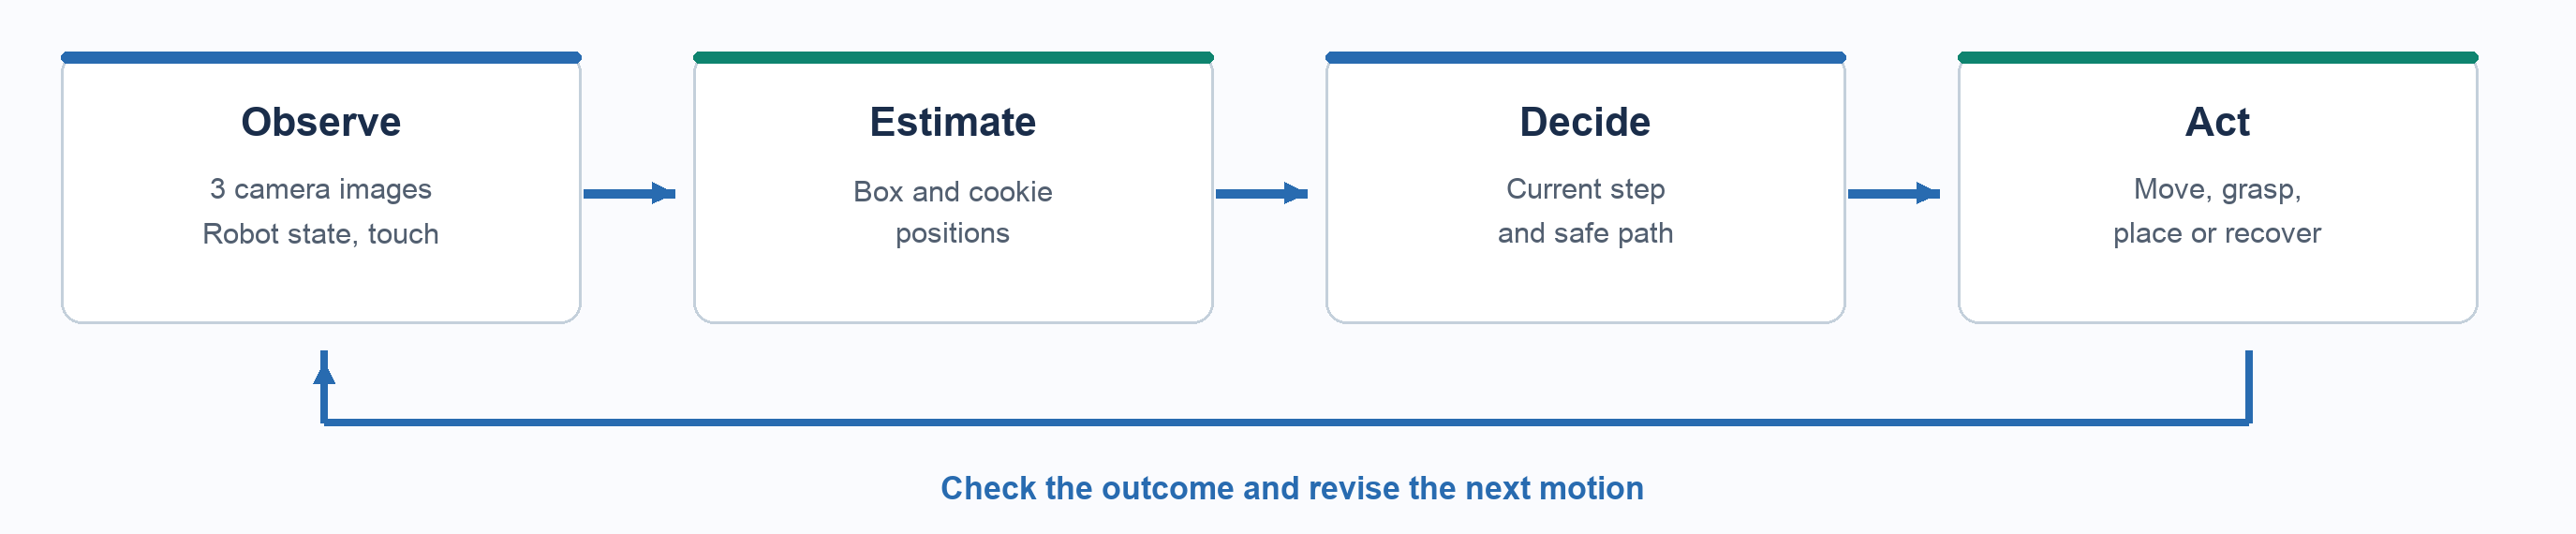
\includegraphics[width=0.99\textwidth]{figures/feedback_controller.png}
\caption{V10's high-level operation. Camera images and public robot measurements are turned into an estimate of the boxes, cookies, and gripper. The controller chooses a movement and checks the next observation before continuing.}
\label{fig:controller}
\end{figure*}

\subsection{Seeing the boxes and the cookies}
The three cameras see different aspects of the same scene. The front view helps locate the source and target boxes; wrist views are useful when the gripper approaches a narrow gap. Our visual estimator uses the known sizes and shapes of the boxes, robot, and cookies to interpret image edges and colored regions. Where the scene changes slightly, it updates the estimated positions rather than relying solely on the initial layout.

This distinction matters at millimeter scale. For example, a cookie may be centered according to the original box coordinates but offset from the actual gap after the camera or box has moved. A small correction at the last moment can decide whether the fingers enter between cookies or push the entire row. We therefore use broad views to find the layout and closer views to refine the final grasp.

\subsection{Moving in understandable stages}
The rule controller keeps track of which step it is performing. Table~\ref{tab:stages} describes the main stages in ordinary terms. There are also short observation and recovery stages when the robot has insufficient evidence to continue safely.

\begin{table}[t]
\centering\small
\caption{The robot's main actions and the feedback used between them.}
\label{tab:stages}
\begin{tabular}{p{1.6cm}p{5.65cm}}
\toprule
Stage & Meaning \\
\midrule
Choose group & Identify the requested number of remaining cookies. \\
Approach & Move the gripper above the group and line it up with the narrow gap. \\
Grasp & Lower the fingers carefully, close them, and check contact. \\
Lift & Raise the group; verify that the cookies followed the gripper. \\
Carry & Move above the target while checking the held group. \\
Place & Lower into a free region, release when supported, and retreat. \\
Check & Confirm progress; if needed, reobserve, correct, or retry. \\
\bottomrule
\end{tabular}
\end{table}

The controller uses robot geometry to convert desired gripper movement into feasible arm motion. In the final release, it returns the simulator's \emph{Cartesian delta} action: a small change in end-effector position, orientation, and gripper command, rather than an image or a neural-network prediction.

\subsection{Checking contact and carrying}
The first motion after closing the fingers is a cautious lift. Images and force signals help the controller distinguish a real grasp from fingers touching a nearby surface. While carrying, it estimates the group relative to the gripper. If the group slips, the robot should not continue toward a target position calculated for the old grip.

A useful example occurred during development: the robot visibly picked up cookies but carried them about 2--3\,mm away from the assumed position. The same error could later place one edge on the target rim. We addressed such failures by checking the \emph{held object as it is}, not just the gripper pose that was requested.

\subsection{Making room for the next group}
A successful placement has two parts. The current group must fit inside the target, and the robot must be able to open its fingers and withdraw without hitting earlier cookies. In \pTen, the first placement must also leave a reasonable route for the second group. V8--V10 increasingly accounted for these neighboring objects and the changing target layout instead of treating each drop as independent.

This is where several common failures came from: a place looked empty in one view but was blocked by previously placed cookies; an old image was used after the box moved; or the gripper could approach a nominal target point but had no safe way to retreat. The policy therefore links placement decisions to the space occupied by the \emph{whole held group and fingers}, not only to the center of a cookie.

\subsection{Remembering progress and recovering}
The controller tracks the requested batch sizes and how much of the job appears complete. When observations disagree, it may take a better view or return to an earlier step. Later versions added more careful handling of unknown outcomes, a moved box, and a group that was lifted or placed imperfectly.

For example, if a group has already arrived near the target, repeatedly returning to the source to pick it again can create an error. Conversely, counting a group as placed merely because the fingers opened can miss cookies resting on an edge. An explicit account of the groups, their likely locations, and the remaining planned work is essential to deciding the next action.

\paragraph{Why use rules here?}
The task provides well-defined objects and known robot geometry. This lets us express many actions directly: where the fingers should go, when to move slowly, what a safe approach looks like, and when the visual evidence is too weak. The policy is interpretable: a failed run can often be traced to a wrong visual estimate, an unsafe movement, or an incorrect stage transition. Improving these pieces is the focus of the next section.
